\documentclass{beamer}
\usetheme{Singapore}

\usepackage{amsmath,amssymb,latexsym}
\usepackage{graphicx}
\usepackage{fancyvrb}
\usepackage{hyperref}
\usepackage{tikz}

\newcommand{\bi}{\begin{itemize}}
\newcommand{\ii}{\item}
\newcommand{\ei}{\end{itemize}}
\newcommand{\Show}[1]{\psshadowbox{#1}}

\newcommand{\set}[1]{\ensuremath{\left\{ #1 \right\}}}
\newcommand{\nats}{\ensuremath{\mathbb{N}}}
\newcommand{\nni}{\ensuremath{\mathbb{N}^0}}
\newcommand{\ints}{\ensuremath{\mathbb{Z}}}
\newcommand{\power}{\ensuremath{\mathcal{P}}}
\renewcommand{\neg}{\sim}
\newcommand{\xor}{\oplus}
\newcommand{\then}{\ensuremath{\Rightarrow}}
\newcommand{\lcm}{\mbox{lcm}}
\newcommand{\QED}{\hfill\ensuremath{\blacksquare}}
\newcommand{\equivmod}[3]{#1 \equiv #2\ (\mbox{mod } #3)}
\newcommand{\nequivmod}[3]{#1 \not\equiv #2\ (\mbox{mod } #3)}

\newcommand{\grf}[2]{\centerline{\includegraphics[width=#1\textwidth]{#2}}}
\newcommand{\tw}{\textwidth}
\newcommand{\bc}{\begin{columns}}
\newcommand{\ec}{\end{columns}}
\newcommand{\cc}[1]{\column{#1\textwidth}}

\newcommand{\bfr}[1]{\begin{frame}[fragile]\frametitle{{ #1 }}}
\newcommand{\efr}{\end{frame}}

\newcommand{\cola}[1]{\begin{columns}\begin{column}{#1\textwidth}}
\newcommand{\colb}[1]{\end{column}\begin{column}{#1\textwidth}}
\newcommand{\colc}{\end{column}\end{columns}}

\title{Book of Proof: Part IV, Relations, Functions, and Cardinality}

\RecustomVerbatimEnvironment{Verbatim}{Verbatim}{frame=single}

\begin{document}
\begin{frame}
\maketitle

\end{frame}

\bfr{Relations}
\[
\begin{array}{ccc}
  5 < 10 & 3 < 12 & 99 < 999 \\\\
  5 \not< 5 & 12\not< 3 & 10 \not< 0
\end{array}
\]

\pause\vfill
\[ R = \set{(5,10), (3,12), (99,999), \ldots} \]

\[
\begin{array}{ccc}
  (5,10)\in R & (3,12)\in R & (99,999)\in R \\\\
  (5,5) \not\in R & (12,3) \not\in R & (10,0)\not\in R
\end{array}
\]


\end{frame}

\bfr{Relations}

{\bf Definition 11.1}  A {\bf relation} on a set $A$ is a subset
$R\subseteq A\times A$.

We abbreviate $(x,y)\in R$ as $xRy$.

\end{frame}


\bfr{Relations in Pictures}

\begin{align*}
  B &=\set{0,1,2,3,4,5} \\
 U &= \set{
  (1,3), (3,3), (5,2), (2,5), (4,2)
} \subseteq B\times B
\end{align*}

\grf{0.5}{relationUonB.png}

\end{frame}

\bfr{Properties of Relations}

{\bf Definition 11.2}  Suppose $R$ is a relation on set $A$.

\begin{enumerate}
\item  $R$ is {\bf reflexive} if $xRx$ for every $x\in A$.
  \[ \forall x\in A, xRx \]

\item $R$ is {\bf symmetric} if $xRy$ implies $yRx$ for all
  $x,y\in A$.
  \[ \forall x,y \in A, xRy \then yRx \]

\item $R$ is {\bf transitive} if $xRy$ and $yRz$ imply $xRz$.
  \[
  \forall x,y,z\in A, ((xRy) \land (yRz)) \then xRz
  \]
\end{enumerate}
\end{frame}

\bfr{Pictures of Relation Properties}

\grf{1.0}{relationpics.png}

\end{frame}


\bfr{Relations on \ints}

\grf{1.0}{relationsonZ.png}


\end{frame}

\bfr{Equivalence relations}

{\bf Definition 11.3}  A relation $R$ on a set $A$ is an {\bf
  equivalence relation} if it is reflexive, symmetric,  and
transitive.

\pause\vfill

{\bf Definition 11.4} Suppose $R$ is an equivalence relation on set
$A$. Given any element $a\in A$, the {\bf equivalence class containing
  $a$} is the subset $\set{x\in A : xRa}$ of $A$ consisting of all
elements of $A$ that relate to $a$.

This set is denoted $[a]$:
\[
  [a] = \set{x \in A : xRa}
  \]
  
\end{frame}


\bfr{Pictures of equivalence relations on $\{-1,1,2,3,4\}$}

\grf{1.0}{equivalencepics.png}

\end{frame}

\bfr{Congruence as equivalence relations}

Example 11.8 proved that $\equivmod{}{}{n}$ is an equivalence relation.


\begin{align*}
xRy &= \set{(x,y) : \equivmod{x}{y}{3}} \\\\
[0] &= \set{x\in\ints : \equivmod{x}{0}{3}} \\
&=  \set{x\in\ints : 3\mid (x-0)}
=  \set{x\in\ints : 3\mid x}\\
&= \set{...,-6,-3,0,3,6,9,...} = [3] = [6]\\
[1] &= \set{x\in\ints : \equivmod{x}{1}{3}} \\
&=  \set{x\in\ints : 3\mid (x-1)}\\
&= \set{...,-5,-2,1,4,7,10,...} = [4] = [7]\\
[2] &= \set{x\in\ints : \equivmod{x}{2}{3}} \\
&=  \set{x\in\ints : 3\mid (x-2)}\\
&= \set{...,-4,-1,2,5,8,11,...} = [5] = [7]\\
\end{align*}

\end{frame}

\bfr{Partitions}

{\bf Definition 11.5}  A {\bf partition} of a set $A$ is a set of
non-empty subsets of $A$, such that the union of all the subsets
equals $A$, and the intersection of any two different subsets is
$\emptyset$.

\vfill

$\set{[0],[1],[2]}$ under the relation $\equivmod{}{}{3}$, is a
partition of $\ints$:
\begin{align*}
\set{[0],[1],[2]} &= \{\set{...,0,3,6,...},
\set{...,1,4,7,...},
\set{...,2,5,8,...}\}
\end{align*}

\end{frame}

\bfr{Equivalence Relations and Partitions}

{\bf Theorem 11.2}  Suppose $R$ is an equivalence relation on set
$A$.  The the set $\set{[a] : a\in A}$ of equivalence classes of $R$
forms a partition of $A$.


\vfill

Conversely, any partition of $A$ describes an equivalence relation $R$
where $xRy$ if and only if $x$ and $y$ belong to the same set in the
partition.
\end{frame}


\bfr{The Integers Modulo $n$}

\grf{1.0}{intsmodfive.png}

\[ \ints_5 = \set{[0],[1],[2],[3],[4]} \]

\end{frame}

\bfr{Relations Between Sets}

{\bf Definition 11.7}  A {\bf relation} from a set $A$ to a set $B$ is
a subset $R\subseteq A\times B$.

We abbreviate the statement $(x,y)\in R$ as $xRy$.

\grf{0.5}{relationbetweenAandB.png}

\end{frame}

\bfr{Functions}

{\bf Definition 12.1}  Suppose $A$ and $B$ are sets.  A {\bf function}
from $A$ to $B$ (denoted as $f : A\rightarrow B$) is a relation
$f\subseteq A\times B$, satisfying the property that for each $a\in
A$, the relation $f$ contains exactly one ordered pair of the form
$(a,b)$.  The statement $(a,b)\in f$ is abbreviated $f(a)=b$.

\end{frame}

\bfr{Relations that are functions}

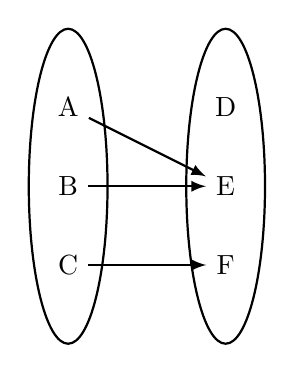
\begin{tikzpicture}[>=latex,thick]
\draw (1,2) ellipse (.5 and 2);
\draw (3,2) ellipse (.5 and 2);
\node (A) at (1,3) {A};
\node (B) at (1,2) {B};
\node (C) at (1,1) {C};
\node (D) at (3,3) {D};
\node (E) at (3,2) {E};
\node (F) at (3,1) {F};
\draw[->] (A) -- (E);
\draw[->] (B) -- (E);
\draw[->] (C) -- (F);
\end{tikzpicture}\hfill
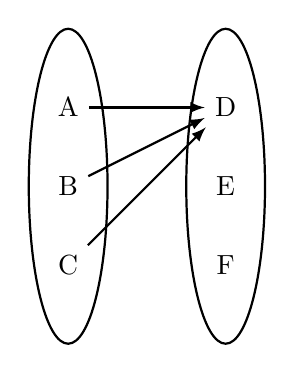
\begin{tikzpicture}[>=latex,thick]
\draw (1,2) ellipse (.5 and 2);
\draw (3,2) ellipse (.5 and 2);
\node (A) at (1,3) {A};
\node (B) at (1,2) {B};
\node (C) at (1,1) {C};
\node (D) at (3,3) {D};
\node (E) at (3,2) {E};
\node (F) at (3,1) {F};
\draw[->] (A) -- (D);
\draw[->] (B) -- (D);
\draw[->] (C) -- (D);
\end{tikzpicture}\hfill
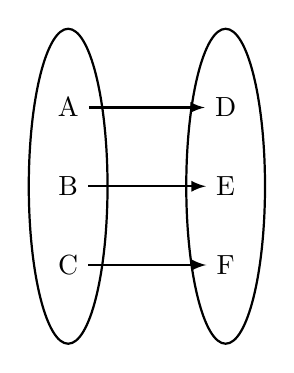
\begin{tikzpicture}[>=latex,thick]
\draw (1,2) ellipse (.5 and 2);
\draw (3,2) ellipse (.5 and 2);
\node (A) at (1,3) {A};
\node (B) at (1,2) {B};
\node (C) at (1,1) {C};
\node (D) at (3,3) {D};
\node (E) at (3,2) {E};
\node (F) at (3,1) {F};
\draw[->] (A) -- (D);
\draw[->] (B) -- (E);
\draw[->] (C) -- (F);
\end{tikzpicture}



\end{frame}

\bfr{Relations that are {\bf not} functions}

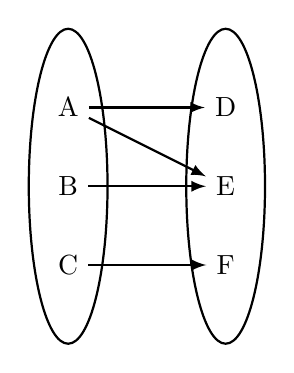
\begin{tikzpicture}[>=latex,thick]
\draw (1,2) ellipse (.5 and 2);
\draw (3,2) ellipse (.5 and 2);
\node (A) at (1,3) {A};
\node (B) at (1,2) {B};
\node (C) at (1,1) {C};
\node (D) at (3,3) {D};
\node (E) at (3,2) {E};
\node (F) at (3,1) {F};
\draw[->] (A) -- (E);
\draw[->] (A) -- (D);
\draw[->] (B) -- (E);
\draw[->] (C) -- (F);
\end{tikzpicture}\hfill
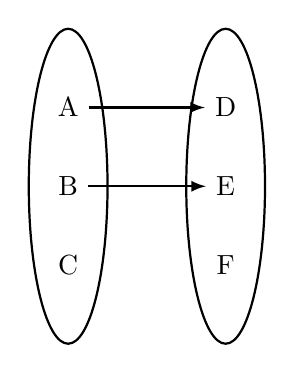
\begin{tikzpicture}[>=latex,thick]
\draw (1,2) ellipse (.5 and 2);
\draw (3,2) ellipse (.5 and 2);
\node (A) at (1,3) {A};
\node (B) at (1,2) {B};
\node (C) at (1,1) {C};
\node (D) at (3,3) {D};
\node (E) at (3,2) {E};
\node (F) at (3,1) {F};
\draw[->] (A) -- (D);
\draw[->] (B) -- (E);
\end{tikzpicture}\hfill
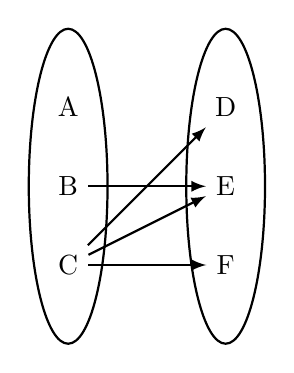
\begin{tikzpicture}[>=latex,thick]
\draw (1,2) ellipse (.5 and 2);
\draw (3,2) ellipse (.5 and 2);
\node (A) at (1,3) {A};
\node (B) at (1,2) {B};
\node (C) at (1,1) {C};
\node (D) at (3,3) {D};
\node (E) at (3,2) {E};
\node (F) at (3,1) {F};
\draw[->] (C) -- (D);
\draw[->] (C) -- (E);
\draw[->] (C) -- (F);
\draw[->] (B) -- (E);
\end{tikzpicture}




\end{frame}
\bfr{Domain, Codomain, Range}

{\bf Definition 12.2}

For a function $f:A\rightarrow B$, the set $A$
is called the {\bf domain} of $f$.

The set $B$ is called the {\bf
  codomain} of $f$.

The {\bf range} of $f$ is the set
$
\set{f(a) :  a\in A} = \set{b : (a,b)\in f}
$.

\end{frame}
\bfr{Example function}

\begin{align*}
  A &= \set{p,q,r,s}\\
  B &= \set{0,1,2}\\
  f &= \set{(p,0),(q,1),(r,2),(s,2) }
\end{align*}

\grf{1.0}{funcfromatob.png}

\end{frame}

\bfr{Example function}
\begin{align*}
  f(x) &= x^2 \\\\
  f &= \lambda x . x^2\\\\
  f &= \set{(x,x^2) : x \in \mathbb{R}}
\end{align*}
\vfill\pause
Not complete definition unless you specify domain and codomain:
\[ f : \mathbb{R} \rightarrow \mathbb{R} \]

\end{frame}

\bfr{Example function}
\begin{align*}
  \phi &: \ints^2 \rightarrow \ints\\\\
  \phi(m,n) &= 6m-9n\\\\
  \phi &= \set{((m,n),6m-9n) : (m,n)\in\ints^2}\\
  &= \set{((0,0),0), ((1,1),-3), ((1,0), 6), ...}\\
  &\subseteq \ints^2 \times \ints
\end{align*}

\pause
\begin{itemize}
\item  What is the domain? \pause $\mathbb{Z^2}$
\item What is the codomain? \pause $\mathbb{Z}$
\item What is the range? \pause $\set{3k : k\in\ints} $
\end{itemize}

\end{frame}

\bfr{Equality of functions}

{\bf Definition 12.3} Two functions $f : A\rightarrow B$ and $g :
C\rightarrow D$ are {\bf equal} if $A=C$, $B=D$, and $f(x)=g(x)$ for
every $x\in A$.

\end{frame}

\bfr{Injections and Surjections}

{\bf Definition 12.4}  A function $f : A\rightarrow B$ is
\begin{enumerate}
  \item {\bf injective} (or one-to-one) if\\ for every $x,y\in A$,
    $x\neq y \then f(x) \neq f(y)$;
  \item {\bf surjective} (or onto) if\\ for every $b\in B$ there is an
    $a\in A$ with $f(a) = b$;
  \item {\bf bijective} if $f$ is both injective and surjective.
\end{enumerate}

\grf{1.0}{injectionsurjection.png}
\end{frame}

\bfr{Injective and Surjective Examples}
\grf{1.0}{injsurjexamples.png}
\end{frame}

\bfr{Proving a function is an injection}
    {\bf How to show a function $f:A\rightarrow B$ is injective:}

    \fbox{\parbox{0.45\textwidth}{
        {\bf Direct approach:}

        Suppose $x,y\in A$, $x\neq y$.

        $\vdots$

        Therefore $f(x)\neq f(y)$.
        }}\hfill
    \fbox{\parbox{0.5\textwidth}{
        {\bf Contrapositive approach:}

        Suppose $x,y\in A$, $f(x)=f(y)$.

        $\vdots$

        Therefore $x=y$.
    }}

\vfill
    Contrapositive is usually easier.

    \vfill

    {\bf How to show a function $f:A\rightarrow B$ is not injective:}
    \fbox{\parbox{0.9\textwidth}{
      Find $x,y\in A, x=y$, with $f(x)\neq f(y)$.}}


\end{frame}

\bfr{Proving a function is a surjection}

{\bf How to show a function $f:A\rightarrow B$ is surjective:}

\fbox{\parbox{0.9\textwidth}{
    Suppose $b\in B$.

    $\vdots$

    There exists $a\in A$ with $f(a) = b$.
}}

\vfill

{\bf How to show a function $f:A\rightarrow B$ is not surjective:}

\fbox{\parbox{0.9\textwidth}{
    Find $b\in B$ such that
    for all $a\in A, f(a) \neq b$.
}}




\end{frame}

\bfr{Example 12.4}

{\bf Proposition}
$f:\mathbb{R}-\set{0} \rightarrow \mathbb{R}$ defined as
$f(x)=\frac{1}{x} + 1$ is injective but not surjective.
\vfill

{\bf Injective.} \pause  Suppose $x,y\in\mathbb{R}-\set{0}$ and $f(x)=f(y)$.

This implies $\frac{1}{x} + 1 = \frac{1}{y} + 1$.

Algebra shows $x=y$.  Therefore $f$ is injective.
\vfill
{\bf Not surjective.} \pause There exists $b=1\in\mathbb{R}$ for which $f(x)
=\frac{1}{x} + 1\neq 1$ for every $x\in\mathbb{R}-\set{0}$.

\end{frame}


\bfr{Example 12.5}

{\bf Proposition}  The function
$g:\ints\times\ints\rightarrow\ints\times\ints$ defined by
$g(m,n) = (m+n,m+2n)$ is both injective and surjective.

\vfill

{\bf Injective.} \pause  Suppose $(m,n), (k,\ell)\in\ints\times\ints$
and $g(m,n) = g(k,\ell)$.

Then $(m+n,m+2n) = (k+\ell,k+2\ell)$.

Then $m+n=k+\ell$ and $m+2n=k+2\ell$.

Algebra shows $m=k$ and $n=\ell$.

Therefore $(m,n)=(k,\ell)$ and $g$
is injective.

\vfill

{\bf Surjective.} \pause Suppose $(b,c)\in\ints\times\ints$.

We need to find $(x,y)\in\ints\times\ints$ for which $g(x,y)=(b,c)$.

We need to find $(x,y)$ such that $x+y=b$ and $x+2y=c$.

Solving gives $x=2b-c$ and $y=c-b$.

Therefore $g(2b-c,c-b) = (b,c)$ and so $g$ is surjective.

\end{frame}

\bfr{The Pigeonhole Principle}

Suppose $A$ and $B$ are finite sets and $f:A\rightarrow B$ is any
function.
\begin{enumerate}
\item If $|A| > |B|$ then $f$ is not surjective.
\item If $|A| < |B|$ then $f$ is not surjective.
\end{enumerate}

\vfill
\grf{1.0}{pigeonholes.png}
\end{frame}

\bfr{Pigeonhole Principle Example}

{\bf Proposition}  If $A$ is any set of 10 integers between 1 and 100,
then there exist two different subsets $X,Y\subseteq A$ for which the
sum of elelments in $X$ equals the sum of elements in $Y$.

{\bf Examples}
\begin{align*}
  A &= \set{ 5, 11, 16, 23, 44, 47, 50, 61, 67, 81}\\
  X &= \set{5,11,16,23}\\
  Y &= \set{5,50}
\end{align*}
\begin{align*}
  A &= \set{ 5, 12, 16, 23, 44, 47, 50, 61, 67, 81}\\
  X &= \set{5,12,16,23}\\
  Y &= \set{12,44}
\end{align*}


\end{frame}

\bfr{Pigeonhole Principle Example}

{\bf Proposition}  If $A$ is any set of 10 integers between 1 and 100,
then there exist two different subsets $X,Y\subseteq A$ for which the
sum of elelments in $X$ equals the sum of elements in $Y$.

\vfill

{\it Proof.}  Suppose $A$ is as stated and $X\subseteq A$.

Then $X$ has no more than 10 elements between 1 and 100, so the sum of
all elements in $X$ is less than 1000.

How many subsets of $A$ are there?

\pause

\[ |\mathcal{P}(A)| = 2^{10} = 1024 \]

\pause
By the pigeonhole principle, two of these sets must have the same sum.


\end{frame}

\bfr{Pigeonhole Principle Example}

{\bf Proposition} There are at least two people in Washington State
with the same number of hairs on their heads.

\vfill\pause

{\it Proof.}

The population of Washington is more than seven million.

Every human head has fewer than one million hairs.

By the pigeonhole principle, two Washingtonians must have the same
number of hairs on their head.

\end{frame}

\bfr{Composition}

{\bf Definition 12.5}  Suppose $f:A\rightarrow B$ and $g:B\rightarrow
C$ are functions with the property that the codomain of $f$ is the
domain of $g$.  The {\bf composition} of $f$ with $g$, denoted $g\circ
f$, is defined as follows.

For all $x\in A$:
\[ g\circ f(x) = g(f(x)) \]

\grf{0.5}{composition.png}

\end{frame}

\bfr{Inverse Functions}

{\bf Definition 12.6}  Given a set $A$, the {\bf identity function} on
$A$ is the function $i_A(x)=x$ for all $x\in A$.
\vfill

{\bf Definition 12.7}  Given a relation $R$ from $A$ to $B$, the {\bf
  inverse relation} of $R$ is the relation from $B$ to $A$ defined as
\[ R^{-1} = \set{(y,x) : (x,y)\in R} \]

\end{frame}

\bfr{Example Inverses}
\grf{0.75}{inversef}
\grf{0.75}{inverseg}
\vfill

$f, g, f^{-1}$ are functions.
\hfill
$g^{-1}$ is not a function.


\end{frame}

\bfr{Function Inverses}

{\bf Theorem 12.3}  Let $f: A\rightarrow B$ be a function.

$f$ is
bijective if and only if the inverse relation $f^{-1}$ is a function
from $B$ to $A$.

\end{frame}

\bfr{Image and Preimage}

{\bf Definition 12.9}  Suppose $f:A\rightarrow B$ is a function.
\begin{enumerate}
\item If $X\subseteq A$ the {\bf image} of $X$ is the set
  \[ f(X) = \set{f(x) : x\in X} \subseteq B \]
\item If $Y\subseteq B$ the {\bf preimage} of $Y$ is the set
  \[ f^{-1}(Y) = \set{x\in A : f(x) \in Y} \]
\end{enumerate}
\vfill

Note that $f$ denotes two functions:
\begin{description}
\item $f:A\rightarrow B$
\item  $f:\mathcal{P}(A)\rightarrow \mathcal{P}(B)$
\end{description}

Note that $f^{-1}(X)$ is a function even if $f$ is not invertible:
\begin{description}
\item  $f^{-1}:\mathcal{P}(B)\rightarrow \mathcal{P}(A)$
\end{description}

\end{frame}

\bfr{Cardinality}

{\bf Definition 13.1}  Two sets $A$ and $B$ have the {\bf same
  cardinality}, written $|A| = |B|$, if there exists a bijective
function $f:A\rightarrow B$.
\vfill

\grf{1.0}{nobijection}

\end{frame}

\bfr{$|\ints| = |\nats|$}

{\huge
\begin{tabular}{c|cccccccccc}
\nats&  1&2&3&4&5&6&7&8&9&...\\\hline
\ints&  0  &1&-1&2&-2&3&-3&4&-4&...
\end{tabular}
}

\end{frame}

\bfr{$|\nats| \neq |\mathbb{R}|$}

\grf{0.5}{diagonal}

$b= 0.01010001001000...$ is not in the table.
\end{frame}

\bfr{Countable and Uncountable Sets}

{\bf Definition 13.2}  Suppose $A$ is a set.

Then $A$ is {\bf countably infinite} if $|\nats| = |A|$.

$A$ is {\bf uncountable} if $A$ is infinite and $|\nats| \neq |A|$.

$A$ is {\bf countable} if it is finite or countably infinite.

\vfill\pause
{\bf Theorem 13.3} A set $A$ is countably infinite if and only if its
elements can be arranged in an infinite list $a_1, a_2, a_3, a_4,
...$.


\end{frame}

\bfr{The set of rational numbers, $\mathbb{Q}
 = \set{\frac{a}{b} : a\in\ints, b\in\nats}
 $}
\grf{0.8}{rationals}
\end{frame}

\bfr{$\mathbb{Q}$ is countably infinite.}
\grf{0.7}{rationalsnake}
\end{frame}

\bfr{If $A$ and $B$ are countably infinite, then so is $A\times B$}
\grf{0.7}{atimesb}
\end{frame}

\bfr{Comparing cardinalities}

{\bf Definition 13.4}  Suppose $A$ and $B$ are sets.
\begin{enumerate}
\item $|A| = |B|$ means there is a bijection $A\rightarrow B$.
\item $|A| < |B|$ means there is an injection $A\rightarrow B$
  but no surjection.
\item $|A| \leq |B|$ means $|A| < |B|$ or $|A| = |B||$.
\end{enumerate}
\vfill

\grf{1.0}{nobijection}
\end{frame}

\bfr{Size of the power set}

{\bf Theorem 13.7}  If $A$ is any set, then $|A| < |\mathcal{P}(A)|$.

\vfill

{\it Proof.}

{\bf There exists an injection:}

$g(a) = \set{a}$ for $a\in A$ is an injection $A\rightarrow
\mathcal{P}(A)$.

\vfill

{\bf There is no surjection:}

Suppose $f:A\rightarrow\mathcal{P}(A)$ is a surjection.

Let $B = \set{x\in A : x\not\in f(x)} \subseteq A$.

Since $f$ is a surjection, there is $a\in A$ with $f(a) = B$.

{\bf Case 1:} $a\in B$.  Then the definition of $B$ implies $a\not\in
B$.

{\bf Case 2:} $a\not\in B$.  Then the definition of $B$ implies $a\in
B$.

In both cases we have a contradiction, so $f$ cannot be a surjection.
\end{frame}

\bfr{Consequences of Theorem 13.7}

\[
|\nats| < |\mathcal{P}(\nats)|
< |\mathcal{P}(\mathcal{P}(\nats))|
< |\mathcal{P}(\mathcal{P}(\mathcal{P}(\nats)))|
< |\mathcal{P}(\mathcal{P}(\mathcal{P}(\mathcal{P}(\nats))))|
< ...
\]


\end{frame}

\bfr{Some Theorems About Countability}

{\bf Theorem 13.8} An infinite subset of a countably infinite set is
countably infinite.

\vfill

{\bf Theorem 13.9} If $U\subseteq A$ and $U$ is uncountable, then $A$
is uncountable.


\vfill

{\bf Theorem 13.10 (The Cantor-Bernstein-Schroeder Theorem)}

If $|A| \leq |B|$ and $|B|\leq |A|$, then $|A| = |B|$.

In other words, if there are injections $f:A\rightarrow B$ and
$g:B\rightarrow A$, then there is a bijection $h:A\rightarrow B$.

\vfill

{\bf Theorem 13.11}  $|\mathbb{R}| = |\mathcal{P}(\mathbb{N})|$

{\it Proof.}  Uses the CBS theorem.


\end{frame}

\end{document}

